\section{Assignment 5: Scene Recognition with Bag of Visual Words}

The goal of this section is to map any test image to 8 pre-defined scenes described by a training set of images. For this purpose, we try to create a vocabulary of visual words. The goal of a visual word is to be the most expressive descriptor for a type of interest point. As the first step, we use \texttt{vl\_dsift} to get around 100 descriptors from each image on the training collection. We perform k-means clustering on the list of all resulting descriptors to get our visual words. Each visual word therefore is the centroid of a cluster of 128 numbers long SIFT descriptors.


In our tests we utilized both 50 and 75 clusters/visual words.


Once the vocabulary is complete, we need to create a map between the existing training images and our visual words. First we use \texttt{vl\_dsift} to extract the key points of each training image, however this time with a smaller step size. For the exact step size 2 was chosen as the results did not improve with the size of 1. Next we use knnsearch to find the nearest visual word in vocabulary for each SIFT descriptor of the image. Finally we create a (normalized) histogram for each image representing the occurrence count of each visual word in the image. The collection of all histograms(training) and the associated image classes (group) is returned by the function \texttt{BuildKNN}.


The next step is to test images against our model as an attempt to recognize the scene correctly. Again, we use \texttt{vl\_dsift} and create a histogram as described above. As the function \texttt{knnclassify} is removed in MATLAB2018 we used the combination of functions \texttt{fitcknn} and \texttt{predict} to guess the correct scene. The result of the prediction compared to the actual class of the image is reflected by the confusion matrix.

Figures \ref{fig:a5:50c3nn2s} to \ref{fig:a5:75c21nn2s} visualize the precision rate and the confusion matrix for different sizes of vocabulary, step parameter and number of neighbors.


\begin{figure}[h]
	\centering
	\begin{subfigure}{0.3\textwidth}
		\begin{subfigure}[t]{\textwidth}
			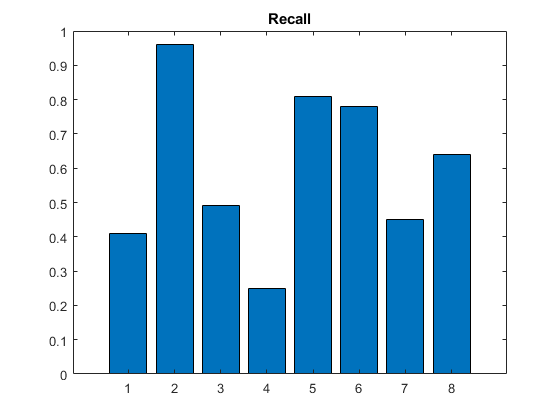
\includegraphics[width=\textwidth]{figures/recall_50C_3NN_2S.png} 
			\caption{Recall}
		\end{subfigure}
		\begin{subfigure}[t]{\textwidth}
			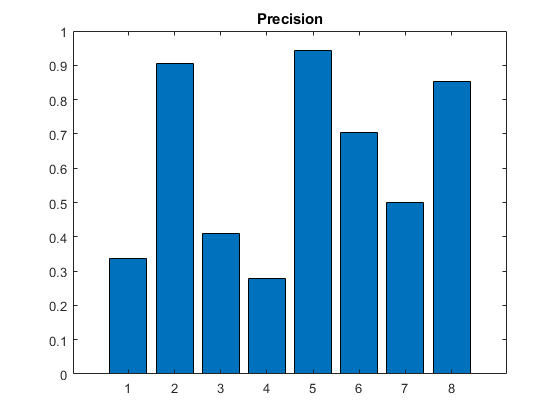
\includegraphics[width=\textwidth]{figures/precision_50C_3NN_2S.png}
			\caption{Precision}
		\end{subfigure}

	\end{subfigure}
	\begin{subfigure}{0.65\textwidth}
		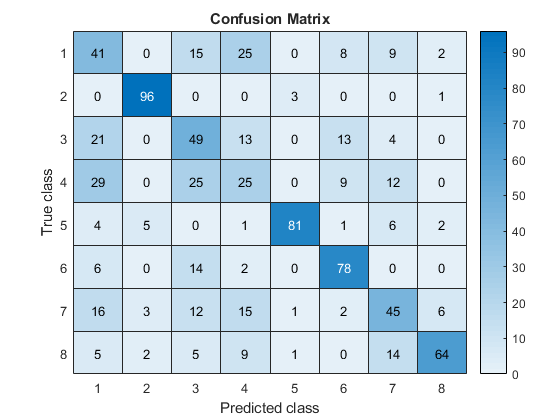
\includegraphics[width=\textwidth]{figures/confusion_50C_3NN_2S.png}
		\caption{Confusion Matrix}
	\end{subfigure}
	\caption{Results for numClusters = 50, numNeighbors = 3 and step size of 2. Success rate is 59.9\%.}
	\label{fig:a5:50c3nn2s}
\end{figure}

\begin{figure}[h]
	\centering
	\begin{subfigure}{0.3\textwidth}
		\begin{subfigure}[t]{\textwidth}
			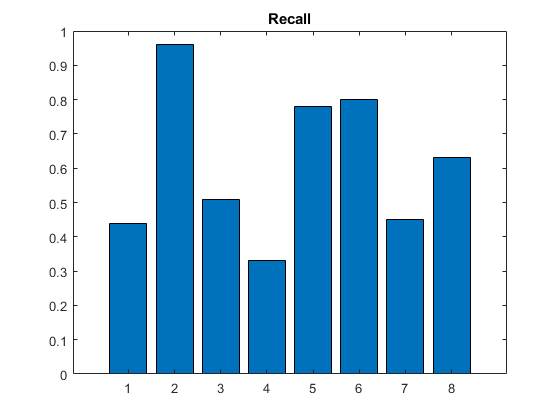
\includegraphics[width=\textwidth]{figures/recall_75C_3NN_2S.png} 
			\caption{Recall}
		\end{subfigure}
		\begin{subfigure}[t]{\textwidth}
			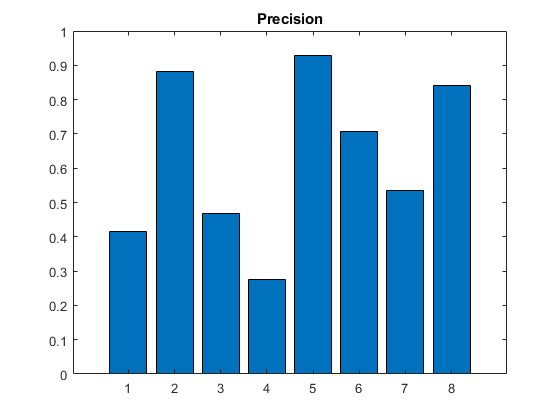
\includegraphics[width=\textwidth]{figures/precision_75C_3NN_2S.png}
			\caption{Precision}
		\end{subfigure}

	\end{subfigure}
	\begin{subfigure}{0.65\textwidth}
		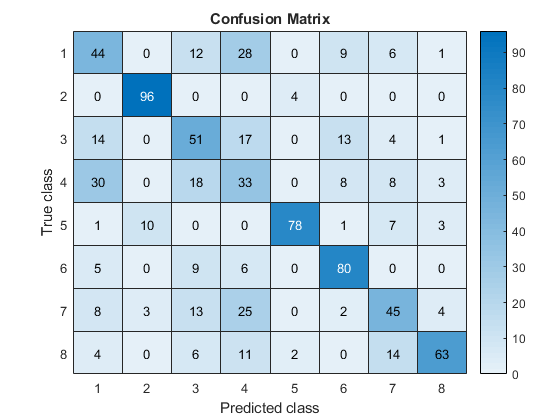
\includegraphics[width=\textwidth]{figures/confusion_75C_3NN_2S.png}
		\caption{Confusion Matrix}
	\end{subfigure}
	\centering
	\caption{Results for numClusters = 75, numNeighbors = 3 and step size of 2. Success rate is 61.3\%.}
	\label{fig:a5:75c3nn2s}
\end{figure}

\begin{figure}[h]

	\centering
	\begin{subfigure}{0.3\textwidth}
		\begin{subfigure}[t]{\textwidth}
			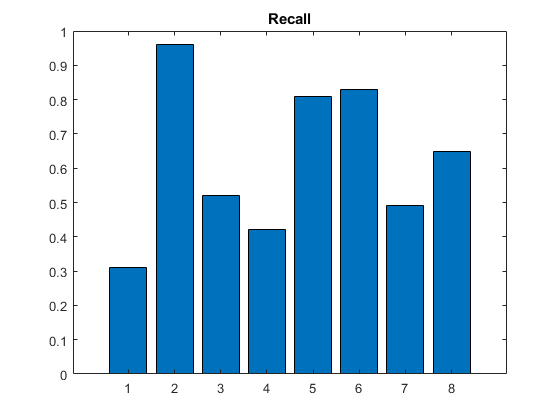
\includegraphics[width=\textwidth]{figures/recall_75C_5NN_2S.png} 
			\caption{Recall}
		\end{subfigure}
		\begin{subfigure}[t]{\textwidth}
			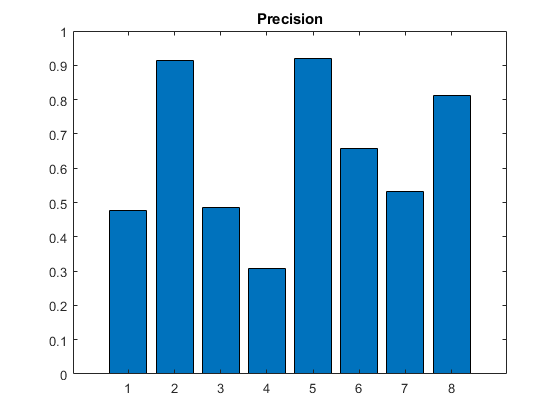
\includegraphics[width=\textwidth]{figures/precision_75C_5NN_2S.png}
			\caption{Precision}
		\end{subfigure}

	\end{subfigure}
	\begin{subfigure}{0.65\textwidth}
		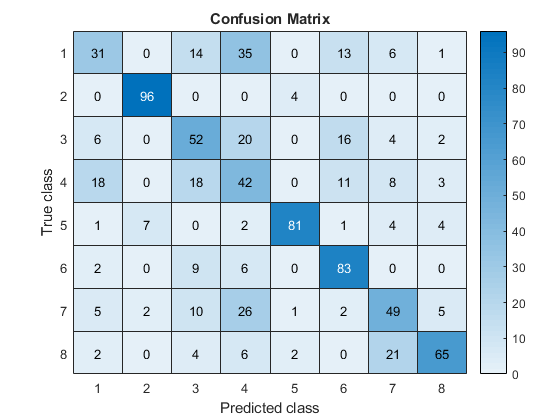
\includegraphics[width=\textwidth]{figures/confusion_75C_5NN_2S.png}
		\caption{Confusion Matrix}
	\end{subfigure}
	\caption{Results for numClusters = 75, numNeighbors = 5 and step size of 2. Success rate is 62.4\%.}
	\label{fig:a5:75c5nn2s}
\end{figure}

\begin{figure}[h]
	\centering
	\begin{subfigure}{0.3\textwidth}
		\begin{subfigure}[t]{\textwidth}
			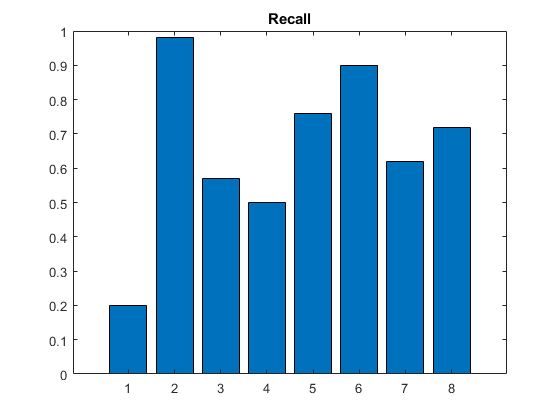
\includegraphics[width=\textwidth]{figures/recall_75C_21NN_2S.png} 
			\caption{Recall}
		\end{subfigure}
		\begin{subfigure}[t]{\textwidth}
			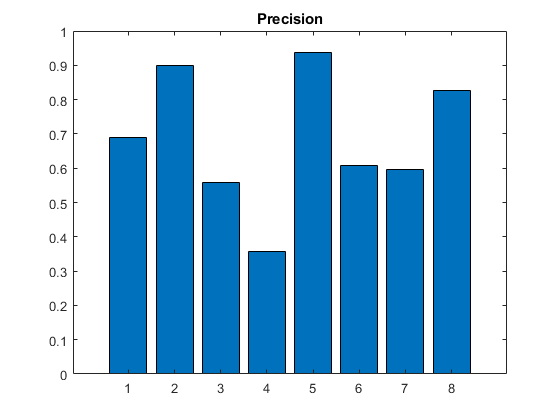
\includegraphics[width=\textwidth]{figures/precision_75C_21NN_2S.png}
			\caption{Precision}
		\end{subfigure}

	\end{subfigure}
	\begin{subfigure}{0.65\textwidth}
		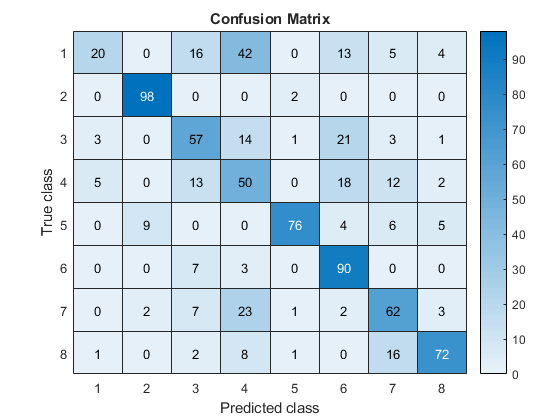
\includegraphics[width=\textwidth]{figures/confusion_75C_21NN_2S.png}
		\caption{Confusion Matrix}
	\end{subfigure}

	\caption{Results for numClusters = 75, numNeighbors = 21 and step size of 2. Success rate is 65.6\%.}
	\label{fig:a5:75c21nn2s}
\end{figure}

As illustrated by the diagrams, the success rates of the classes mountain, forest and street is quite high. The classes bedroom, kitchen and living room have a high rate of confusion with each other. Especially the living room's bad detection rate is mostly due to the other 2 categories. There is a certain confusion between mountain and forest, however that can be seen as expected.

// self test images